\chapter{Métodos y materiales}

En este capítulo se mostrarán las herramientas matemáticas necesarias para obtener los resultados, se comienza con 
una breve introducción a la generación de números aleatorios. Se describirá el modelo SIS y se relacionará con la teoría de procesos estocásticos;
relativos a estos, hablaremos de la ecuación maestra, la de Fokker-Planck y la de Langevin. Finalmente, se describirá el 
algoritmo de Gillespie.

\section{Generación de números aleatorios}

Necesitamos hacer un pequeño preámbulo a los números aleatorios, ya que tienen un papel fundamental en los métodos Montecarlo, los cuales nos 
permitirán usar estos números aleatorios para obtener soluciones numéricas de nuestros modelos, en particular, a generar variables 
estocásticas a las que les asignaremos una distribución determinada.

Estos métodos dependen de generadores de números pseudoaleatorios, que son algoritmos que nos permiten obtener una secuencia de números
determinista y periódica cuyas propiedades son muy parecidas a una secuencia totalmente aleatoria. Estas secuencias dependen de un valor
inicial, que llamaremos ``semilla''. En muchos casos la elección de esta es fundamental porque la ``calidad'' de los números obtenidos
puede depender del valor inicial.

En este trabajo se han utilizado generadores de números aleatorios implementados en la biblioteca ``numpy''  de Python. Aun así, vamos a 
estudiar algún ejemplo para entender los fundamentos de dichos métodos.

\newpage

\subsection{Generadores de números pseudoaleatorios uniformes}
Uno de los primeros métodos descubiertos es el generador lineal congruencial, para un estudio más profundo véase el Anexo A de \cite{Toral}. Mediante 
este método se obtienen enteros aleatorios que llamaremos $x\in [0,M-1]$. Donde $M$ es el entero que actuará como cota superior. De forma general
es interesante que $M$ sea un número grande, ya que si hacemos el cambio de variable $x/M$ obtendremos números cuasiuniformes en el intervalo $[0,1]$,
que es la base de muchos otros, como el método de la transformada inversa que discutiremos posteriormente.
La secuencia de números está definida por la siguiente relación de recurrencia:
\begin{equation}
    n_k=(a\; n_{k-1}+b)\; mod\: M
\end{equation}
Donde $n_0$ es la semilla y $a$ y $b$ son parámetros, multiplicador e incremento respectivamente. En función de los valores que tomen, obtendremos números
mejor o peor distribuidos uniformemente. Un inconveniente de este método es que es muy sensible a la elección de los parámetros, tanto que puede ser que los
números lleguen a estar correlacionados o que el periodo sea demasiado pequeño, por lo que no tendrían as propiedades de número aleatorio que buscamos.
A continuación, en la figura \ref{f:LGC} podemos encontrar como podemos observar como se modifica la distribución de números aleatorios para diferentes
valores de los parámetros.


\begin{figure}[H]
    \centering
     \subfigure[Mala elección de parámetros.]{
      \label{f:malos parámetros}
       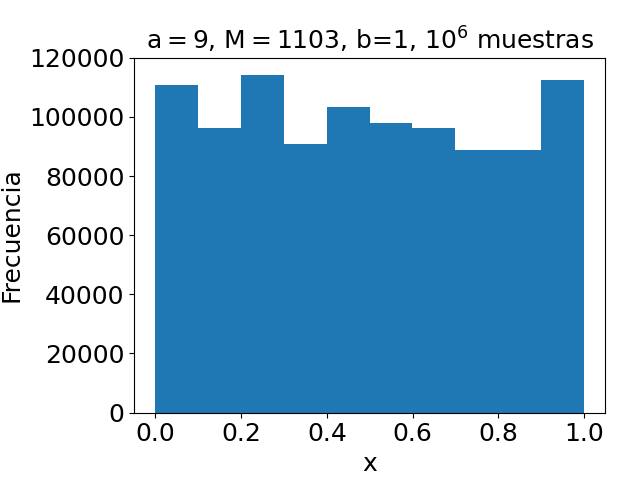
\includegraphics[width=0.47\textwidth]{muestreo malo LGC.png}}
     \subfigure[Buena elección de parámetros.]{
      \label{f:Buenos parámetros}
       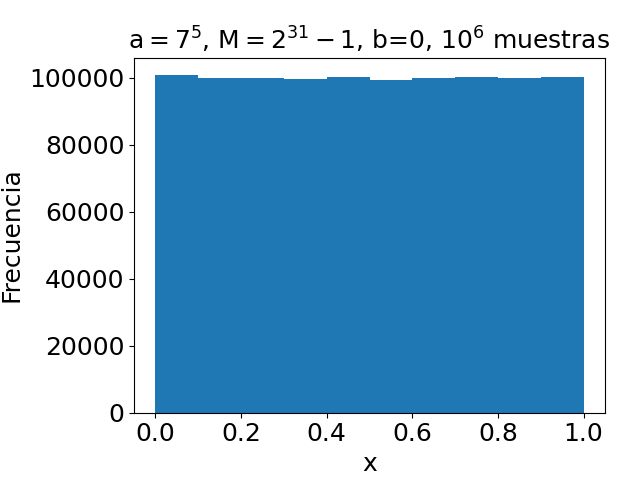
\includegraphics[width=0.47\textwidth]{muestreo bueno LGC.png}}
    \caption{Distribución de los números pseudoaletarios uniformes con el generador lineal congruencial para diferentes valores de los parámetros.}
    \label{f:LGC}
\end{figure}

Para consultar otros valores buenos y malos de estos parámetros, véase \cite{park1988random}.
\newpage
\subsection{Generadores de números pseudoaleatorios no uniformes}
Dependen de los generadores de números uniformes, ya que a partir de estos, aplicándoles otros métodos, lograremos simular las distribuciones
no uniformes. En el caso de la generación de números pseudoaleatorios uniformes, la secuencia de enteros pertenece al intervalo $[0,M-1]$. Sin embargo, será
interesante definir una nueva variable, $u=x/M-1$ de tal forma que $u\in [0,1]$ es una variable cuasicontinua.

Nos centraremos en el método de la transformada inversa, capítulo 2 de \cite{Toral}. Permite obtener un número no uniformemente distribuido por cada número uniformemente
distribuido. El inconveniente de este método es que no siempre podemos encontrar fácilmente la función inversa, por lo que generalmente, tendremos 
que acudir a otros métodos.

Supongamos que queremos obtener una variable $x \in [a,b]$ que esté distribuida como una función cualquiera $p(x)$. Para ello, partimos de una variable cuasicontinua en el intervalo $[0,1]$, de tal forma que $u$ es un número aleatorio que pertenece a este intervalo,
$u\sim U[0,1]$. Tendremos que encontrar el valor de $x$ tal que $P(x)=u$, por lo que podremos despejar $x=P^{-1}(u)$, de esta forma x estará distribuida
como nosotros le pedimos. Se ve a continuación la demostración.

$$p_x(x)=\overbrace{p_u(u)}^{1}\dfrac{du}{dx}=\dfrac{d}{dx}\underbrace{\int_{a}^{x}p(x)^{\prime}dx^{\prime}}_{P(x)}=p(x)$$
A continuación, en la figura \ref{f:diagrama transformada inversa} se muestra un diagrama del método de la transformada inversa.

\begin{figure}[H]
    \centering
    \includegraphics[width=1\textwidth]{Tfg ANTONIO- 2 - fONDO EL otro.png}
    \caption{Diagrama del método de la transformada inversa. (a) Distribución de probabilidad. (b) Probabilidad acumulada.}
    \label{f:diagrama transformada inversa}
\end{figure}
\newpage
En nuestro caso utilizaremos un generador de números aleatorios que sigan una distribución gaussiana, en la figura \ref{f:gauss} 
encontramos dicha distribución obtenida mediante este método.

\begin{figure}[H]
    \centering
    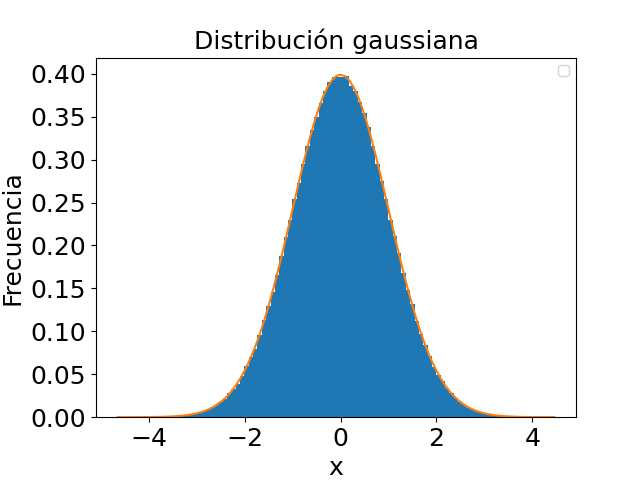
\includegraphics[width=0.65\textwidth]{gauss.png}
    \caption{Muestreo de $10^6$ números aleatorios distribuidos gaussianamente usando el método de la transformada inversa.}
    \label{f:gauss}
\end{figure}



\section{Entorno de programación}

Para la implemetación de los métodos de resolución se ha utilizado el lenguaje Python. Concretamente, se ha utilizado python instalado en Visual Studio Code, que también
ha permitido realizar este documento en formato \LaTeX. Se ha elegido este lenguaje de programación debido a la simplicidad de su sintaxis
lo cual ha hecho su aprendizaje más llevadero. Además, puesto que es uno de los lenguajes en auge en la actualidad \cite{github}, podremos encontrar gran cantidad
de bibliotecas que nos facilitarán el trabajo. En el caso de este trabajo, hemos utilizado las bibliotecas ``numpy'' y ``matplotlib''.

La primera proporciona un amplio abanico de funciones matemáticas, además de un soporte más eficiente para cálculos que el perteneciente a Python
lo que hará que nuestras simulaciones sean más rápidas, algo que nos interesa, ya que cuanto mayor sea la población que queramos analizar, se necesitarán
en general, hacer más cálculos. Además, esta biblioteca incluye generadores de números aleatorios que utilizaremos para resolver las ecuaciones de 
nuestro modelo; también nos permitirá obtener medias y desviaciones de nuestros conjuntos de datos rápidamente.

Por otro lado, la biblioteca matplotlib nos permite graficar los resultados obtenidos, nos hará posible estudiar y analizar la expansión de la epidemia
de manera visual. En general, la combinación de estas dos bibliotecas junto con el lenguaje Python permitirá resolver problemas de manera eficiente
con el uso de un lenguaje de programación sencillo.

Para una descripción más profunda de estas bibliotecas, véase \cite{McKinney} y/o \cite{VanderPlas}.

\section{Modelo SIS}\label{sec:modelo sis}
El modelo que utilizaremos para caracterizar la epidemia es el SIS: susceptible-infectado-susceptible.
Además, consideraremos el caso en el que todos los individuos pueden interactuar con todos y que el número total de individuos no cambia, para un estudio de 
este modelo en redes heterogéneas, véase \cite{Satorras}. 

Bajo este modelo, los individuos pueden estar en dos estados, infectado y susceptible a ser infectado. Como el número de individuos totales que denotamos como $N$
es constante, el estado quedará determinado por el número de infectados $(n_i)$ o susceptibles $(n_s)$, ya que $N=n_i+n_s$.

En este modelo se pueden dar dos interacciones que alteren el estado del sistema. La primera es que un individuo susceptible interaccione con un infectado
y este lo infecte con una probabilidad por unidad de tiempo que denotamos $\lambda$. Podemos esquematizar esta interacción de la siguiente forma:

\begin{equation}
    S+I \;\xrightarrow{\lambda}\;I+I
    \label{eq: infección de susceptible}
\end{equation}

La otra interacción es que un individuo infectado se recupere y pase a volver susceptible, con una probabilidad por unidad de tiempo de ocurrir 
que llamamos $\mu$. El esquema de esta interacción queda:
\begin{equation}
    I \; \xrightarrow{\mu}\;S
    \label{eq: recuperación de un infectado}
\end{equation}

Este es el modelo más simple. Podemos estudiar variantes de este como el SIR, en el que cuando el individuo se recupera no es susceptible 
a infectarse durante un determinado periodo de tiempo, ya que ha adquirido una inmunidad. Para el estudio más detallado de este y otros modelos, diríjase a \cite{Satorras}.

Nosotros estudiaremos el modelo SIS, al que le haremos una pequeña modificación que consiste en introducir un individuo infectado en la población
en el momento en que el número de infectados sea nulo. Esta modificación es consecuencia de que la dinámica del sistema cuando no hay individuos 
infectados se para, ya que no se pueden dar ninguna de las dos interacciones \ref{eq: infección de susceptible} y
\ref{eq: recuperación de un infectado}. En la figura \ref{f:diagrama modelo sis} se muestra un diagrama de las interacciones 
del modelo SIS y el diagrama de fase que obtendremos bajo nuestras consideraciones.

\begin{figure}[H]
    \centering
    \includegraphics[width=\textwidth]{Diagrama SIS.png}
    \caption{Características del modelo SIS. (a) Dinámica del sistema. (b) Diagrama de fase del modelo SIS.}
    \label{f:diagrama modelo sis}
\end{figure}

Como se ve en la figura (b) distinguimos dos fases, la fase absorbente es en la que la $\mu > \lambda$, lo que se traduce en que la probabilidad 
por unidad de tiempo de recuperación es mayor a la de infección, por lo que con el paso del tiempo, se recuperará toda la población y por ello
el número medio de infectados es cero, por lo que es la zona en la que queremos situarnos en la realidad, puesto que aunque existan individuos infectados
en la población, se producirá la recuperación total de estos.

La otra zona es la activa se da cuando $\lambda > \mu$, lo que indica que se producirán más infecciones que recuperaciones con el paso del tiempo. 
Esta es la zona más peligrosa puesto que pese a que el tiempo pase, el número de infectados no bajará naturalmente, sino que se tendrán que poner remedios como el aislamiento para que no se produzcan interacciones o bien tratamientos
médicos que disminuyan la probabilidad de infección para poder volver a la zona absorbente.

Encontramos también un punto crítico cuando $\lambda = \mu$. Aquí es donde es más relevante 
la parte estocástica de nuestro problema, ya que las fluctuaciones del sistema pueden llevarnos a la zona activa o a la absorbente. 
Estas fluctuaciones toman mayor importancia cuanto menor es la población, ya que el cambio de estado de un sistema hace que el porcentaje de
individuos infectados sea mucho mayor o menor relativo a la población total. No es conveniente encontrarnos en esta zona, debido a que es difícil pronosticar
cuál será la evolución de la enfermedad, por lo que es más complicado tomar decisiones para paliar la expansión de esta.




\section{Procesos estocásticos}
Como se ha dicho anteriormente, la evolución de una epidemia es un proceso estocástico, ya que nuestra variable, el número de infectados, evoluciona
de una manera no determinista. Concretamente, se trata de un proceso de Markov \cite{McKane}, en el que la evolución no depende de la
historia pasada del sistema, sino solo del estado en el que se encuentra.


\subsection{Ecuación maestra}
La ecuación maestra es una ecuación diferencial, por lo que es determinista, que describe la evolución de la probabilidad en un proceso de Markov para sistemas que 
pasan de un estado a otro de manera continua en el tiempo \cite{McKane}. Esta ecuación es útil para procesos estocásticos en los que tenemos un número discreto
de estados accesibles, como es nuestro caso. 

Para obtener esta ecuación, denotamos $\vec{n}(t)$ como el estado del sistema y llamamos \newline
$P(\vec{n},t|\vec{n}_0,t_0)$ a la probabilidad de encontrar el sistema en el estado $\vec{n}$ en el tiempo $t$ dadas las condiciones iniciales $\vec{n}(t=t_0)=\vec{n}_0$. Para obtener la 
ecuación maestra, consideraremos que todos los individuos pueden interaccionar con el resto, así no nos tendremos que preocupar de la 
posición de los individuos.

La ecuación maestra es una ecuación de continuidad para el cambio de la probabilidad $P(\vec{n},r|\vec{n}_0,t_0)$ en el tiempo,
por lo que la variación temporal de dicha probabilidad vendrá dada por el flujo de entrada de probabilidad menos el flujo de salida de esta.
Si llamamos $W(\vec{n}\rightarrow \vec{n}^{\prime})$ la probabilidad por unidad de tiempo de pasar del estado $\vec{n}$ al estado $\vec{n}^{\prime}$
la ecuación maestra\footnote{Se ha omitido para no sobrecargar la notación la parte de las condiciones iniciales.} queda:
\begin{equation}
    \dfrac{\partial P(\vec{n},t)}{\partial t}=\sum_{\vec{n}^{\prime}}\left[ W(\vec{n}^{\prime}\rightarrow\vec{n}) P(\vec{n}^{\prime},t) - W(\vec{n}\rightarrow\vec{n}^{\prime}) P( \vec{n}^{\prime},t)\right].
    \label{eq:Ecuación maestra}
\end{equation}

Tendremos un sistema de ecuaciones diferenciales acopladas, una para la probabilidad de cada estado del sistema, 
por lo que solo tendrá solución analítica en muy pocos casos y será costoso de resolver computacionalmente. 
Debido a esto, utilizaremos el algoritmo de Gillespie, ver \ref{sec:Algoritmo de Gillespie}, para obtener trayectorias
compatibles con la solución de esta ecuación. Con este algoritmo obtendremos las trayectorias a partir de la evolución 
de nuestra variable estocástica, el número de infectados.


Vamos a obtener la ecuación maestra del modelo SIS, para posteriormente, tomaremos la aproximación de tamaños grandes, la cual
nos llevará a una ecuación más sencilla de tratar, la ecuación de Fokker-Planck.
Recordamos las posibles interacciones que se pueden dar en el modelo.

\begin{equation*}
    \begin{split}
        S+I\; &\xrightarrow{\lambda}\;I+I\\
        I & \;\xrightarrow{\mu}\;S
    \end{split}
    \label{eq:reacciones}
\end{equation*}

El sistema quedará determinado por el número de individuos infectados, ya que supondremos que la población
es constante, es decir, $N=n_I+n_S$. Para no cargar la notación usaremos $n\equiv n_i$.

Definimos las tasas de probabilidad $W_+$ y $W_-$ de la siguiente manera para poder obtener la ecuación maestra.

\begin{equation}
    \begin{split}
        W_+(n)\equiv& W_{+}(n\rightarrow n+1)=\lambda n(1- \dfrac{n}{N})\\
        W_-(n)\equiv& W_-(n\rightarrow n-1)=\mu n 
    \end{split}
    \label{eq:Reacciones matemática}
\end{equation}

Estas tasas son la probabilidad de un cambio de estado durante un intervalo de tiempo $\Delta t$.
Como se ve en la ecuación \ref{eq:Reacciones matemática}, es la misma expresión que para la colisión de partículas. Producto
de la probabilidad de que se produzca cada uno de los procesos de \ref{eq: infección de susceptible} y \ref{eq: recuperación de un infectado}
multiplicado por el número de individuos en el estado de partida.

De esta forma, la ecuación maestra queda:
\begin{equation}
    \begin{split}
        \partial_t P(n,t)&=W_+(n-1)P(n-1,t)+W_-(n+1)P(n+1,t)-\\
        &-W_-(n)P(n,t)-W_+(n)P(n,t)  
    \end{split}
    \label{eq:Ecuación maestra SIS}
\end{equation}
los dos primeros términos son las probabilidades por unidad de tiempo de que se produzca una interacción que de lugar al estado $(n,t)$.
A este estado se puede llegar a partir del estado $(n-1)$ o desde el estado $(n+1)$, correspondientes al primer y segundo sumando respectivamente.
Los otros dos términos, que están restando, son las probabilidades de que se produzcan interacciones que dan lugar a otro estado.
Partiendo del estado $n$, podremos ir a los estados $(n-1)$ o  al estado $(n+1)$, correspondientes al último y penúltimo sumando respectivamente.
Hacemos el cambio de variable discreta (n) a cuasicontinua (x) adimensionalizando $n$, $x=n/N$. Por lo que las probabilidades cambian también, 
quedando de esta forma $P(n,t)=\tilde{P}(x,t)\dfrac{dx}{dn}=\tilde{P}(x,t)\frac{1}{N}$ y se define también las nuevas tasas $\tilde{W}$ de la siguiente forma:

$$N\tilde{W}_{+}(x,t)=W_{+}(n,t)=\lambda n(1- \dfrac{n}{N})\Longrightarrow\tilde{W}_{+}(x,t)=\lambda x(1-x)$$
$$N\tilde{W}_{-}(x,t)=W_{-}(n,t)=\mu n\Longrightarrow\tilde{W}_{-}(x,t)=\mu x$$

Teniendo en cuesta esto, la ecuación maestra queda:

\begin{equation}
    \begin{split}
        \partial_t\left(\tilde{P}(x,t)\cancel{\dfrac{1}{N}}\right)&=\overbrace{N\tilde{W}_{+}\left(x-\frac{1}{N},t\right)\tilde{P}\left(x-\frac{1}{N},t\right)}^{f\left(x-1/N\right)}\cancel{\dfrac{1}{N}}+\overbrace{N\tilde{W}_{+}\left(x+\frac{1}{N},t\right)\tilde{P}\left(x+\frac{1}{N},t\right)}^{f\left(x+1/N\right)}\cancel{\dfrac{1}{N}}\\
        &-N\tilde{W}_{+}(x,t)\tilde{P}(x,t)\cancel{\dfrac{1}{N}} -N\tilde{W}_{-}(x,t)\tilde{P}(x,t)\cancel{\dfrac{1}{N}}=\\
        &= f\left( x-\frac{1}{N} \right)+f\left( x+\frac{1}{N} \right)-N\tilde{P}(x,t)\left( \tilde{W}_{+}(x)+\tilde{W}_{-}(x) \right)
    \end{split}
    \label{eq:ec fokker}
\end{equation}

\subsection{Ecuación de Fokker-Planck}


Para obtener la ecuación de Fokker-Planck debemos hacer un desarrollo en serie a segundo orden en torno a los puntos $x\pm \frac{1}{N}$ de la nueva función $f$ que hemos definido. Podemos 
aceptar el desarrollo a segundo orden siempre que tengamos una población grande, ya que hacemos el resto de términos los podremos despreciar.

$$f\left(  x\pm \frac{1}{N},t \right)\equiv f\left( x\pm \Delta x,t\right)\simeq f(x,t)\pm \dfrac{1}{N}\partial_x f(x,t)+\dfrac{1}{2N^2}\partial^2_xf(x,t)+\cdots$$

Y la ecuación maestra pasa a ser

\begin{equation}
    \begin{split}
        \partial_t \tilde{P}(x,t)&=\cancel{N\tilde{W}_{+}(x)P(x,t)}-\dfrac{1}{\cancel{N}}\partial_x\left[\cancel{N}\tilde{W}_{+}(x)P(x,t) \right]+\dfrac{1}{2N^{\cancel{2}}}\partial^2_x\left[ \cancel{N}\tilde{W}_{+}(x)P(x,t) \right]+\\
        &+ \cancel{N\tilde{W}_{-}(x)P(x,t)}-\dfrac{1}{\cancel{N}}\partial_x\left[\cancel{N}\tilde{W}_{-}(x)P(x,t) \right]+\dfrac{1}{2N^{\cancel{2}}}\partial^2_x\left[ \cancel{N}\tilde{W}_{-}(x)P(x,t) \right]-\\
        &-\cancel{N\tilde{W}_{+}(x)P(x,t)}-\cancel{N\tilde{W}_{-}(x)P(x,t)}
    \end{split}
\end{equation}

Reagrupando términos y particularizando para nuestras tasas de probabilidad, finalmente obtenemos la ecuación de Fokker-Planck.

\begin{equation}
    \begin{split}
        \partial_t\tilde{P}(x,t)&=-\partial_x\left[ \left( \tilde{W}_{+}-\tilde{W}_{-} \right)\tilde{P}(x,t) \right]+ \dfrac{1}{2N}\partial_x^2\left[ \left( \tilde{W}_{+}+\tilde{W}_{-} \right)\tilde{P}(x,t) \right]\\
        &=-\partial_x\left[ \left( \lambda x (1-x)-\mu x\right)\tilde{P}(x,t) \right]+\dfrac{1}{2N}\partial_x^2\left[ \left( \lambda x (1-x)+\mu x\right)\tilde{P}(x,t) \right]
    \end{split}
    \label{eq:ecuación de Fokker Planck}
\end{equation}

Debido a que es un desarrollo en serie de la ecuación Maestra, la ecuación de Fokker-Planck sigue siendo una ecuación determinista para la
probabilidad, pero en este caso de una variable cuasicontinua. Es por esto que puede ser costosa de resolver tanto analítica como numéricamente,
por lo que de manera análoga a como haremos con el algoritmo de Gillespie, podemos encontrar trayectorias compatibles con la solución de esta 
ecuación. Estas trayectorias las obtendremos resolviendo la ecuación de Langevin, una ecuación diferencial estocástica para la nueva variable
estocástica, el número de infectados normalizado, $x$.


\subsection{Ecuación de Langevin}
Partiendo de la ecuación \ref{eq:ec fokker}, se pueden definir las siguientes funciones:
\begin{equation}
    \begin{split}
        A(x)=&\lambda x (1-x)-\mu x\\
        B(x)=&\lambda x (1-x)+\mu x\\
    \end{split}
    \label{eq:A y B}
\end{equation}
obteniéndose así la siguiente expresión para la ecuación de Fokker-Planck.
$$\partial_t P(x,t)=-\partial_x(A(x)P(x))+\dfrac{1}{2}\partial^2_x(B(x)P(x))$$
\newpage
Podemos ver como se relacionan la ecuación de Langevin y de Fokker-Planck en \cite{McKane,Toral}.
Si realizamos la integración bajo la interpretación de Itô\footnote{Básicamente significa que el ruido ``actúa'' en el momento inicial de cada paso de la integración.}
la ecuación de Langevin pasa a ser:
\begin{equation}
    \dot{x}=A(x)+\sqrt{B(x)}\xi(t)
    \label{eq:Langevin general}
\end{equation}
Donde $\xi(t)$ se denomina ruido blanco gaussiano, \cite{McKane,Toral}. Las principales características de este tipo de ruido son que su media es nula 
y no está correlacionado con él mismo, por lo que su función de autocorrelación es una delta de Kronecker. Físicamente, lo podemos identificar con el límite al continuo de la 
velocidad de una partícula que sigue un movimiento Browniano, es decir, cambia su dirección aleatoriamente y de forma uniforme en el tiempo. 

Como vemos, es una ecuación diferencial estocástica, por lo que será mucho más fácil la integración numérica.

Para nuestro caso, la ecuación queda:

\begin{equation}
        \dot{x}=\lambda x (1-x)-\mu x+\dfrac{1}{\sqrt{N}}\sqrt{\lambda x (1-x)+\mu x} \; \xi(t)    \label{eq:ecuación de langevin}
\end{equation}

Es interesante tomar el límite de población $N\to \infty$, para no encontrar fluctuaciones demográficas.
De esta forma, el segundo término, relacionado con la aleatoriedad de los procesos estocásticos tiende a cero. 
Esto nos permitirá obtener el número medio de infectados una vez alcanzado el estado estacionario.
Para obtener dicho valor, igualamos $\dot{x}=0$, por lo que la ecuación de Langevin queda:

\begin{equation}
    \begin{split}
        \dot{x}=&\lambda x (1-x)-\mu x=0\qquad \textup{Omitimos la solución\footnote{Esto es debido a que esta solución no es estable en la zona activa, que es la que nos interesa estudiar} }x^{est}=0\\ 
        &\lambda(1-x^{est})-\mu=0\\
        &x^{est}=1-\dfrac{\mu}{\lambda}
    \end{split}
    \label{eq: xest}
\end{equation}

\section{Métodos de generación de trayectorias} \label{sec:Algoritmo de Gillespie}

\subsection{Algoritmo de Gillespie}

Como se ha comentado anteriormente, el costo computacional para resolver numéricamente la ecuación maestra es muy alto, es por eso que 
utilizaremos este algoritmo para poder simular trayectorias temporales de la variable estocástica compatibles con la solución de la ecuación maestra.

Para esto, en lugar de estudiar $P(\vec{n},t|\vec{n}_0,t_0)$, estudiaremos una nueva probabilidad, $p(\tau,t|\vec{n},t)$, que se define tal que
$p(\tau,t|\vec{n},t)d\tau$ es la probabilidad de que ocurra la reacción $j$ en el intervalo de tiempo $d\tau$. Esta probabilidad vendrá dada por 
la siguiente expresión \cite{Gillespie}:

\begin{equation}
    P(\tau,\vec{n},t)=\sum_j W_j(\vec{n})\; exp \left( \sum_j W_j\: \tau \right)
\end{equation}

Donde $W_j$ es la probabilidad de que la interacción $j$ se produzca en un intervalo de tiempo $d \tau$

Si sumamos para todos los valores de $j$, obtendremos la probabilidad de que cualquier reacción ocurra en el intervalo de tiempo $d\tau$, que será
la base para obtener las trayectorias compatibles con la solución de la ecuación maestra.
\begin{equation}
    P(\tau|\vec{n},t)=\sum_j W_j(\vec{n})\; exp\left( -\sum_j W_j(\vec{n})\tau\right)
    \label{eq:Gillespie 2}
\end{equation}

Como vemos en la ecuación \ref{eq:Gillespie 2}, $\tau$ se distribuye como una variable aleatoria exponencial de media $W_0(\vec{n}) \equiv \dfrac{1}{ \sum_j W_j (\vec{n})}$
y $j$ es un número entero aleatorio cuya probabilidad es $W_j/W_0$.

Para generar valores de $\tau$ y $j$ compatibles utilizaremos el método directo, el cual se basa en el método de la transformada inversa
mencionado anteriormente. Primero debemos obtener dos enteros aleatorios que llamamos $r_1$ y $r_2$ pertenecientes a la distribución $U(0,1)$. A 
partir de estos obtenemos $\tau$ y $j$:

\begin{equation}
    \begin{split}
        \tau &=\dfrac{1}{W_0(\vec{n})}\:ln \left( \dfrac{1}{r_1} \right)\\
        j&=\textup{el entero más pequeño tal que} \; \; \sum_{j^{\prime}=1}^{j}W_{j^\prime}(\vec{n}) > r_2 W_0(\vec{n}) 
    \end{split}
    \label{eq:generar tau j}
\end{equation}
Una vez obtenidos, el algoritmo que tenemos que realizar es el siguiente:
\begin{enumerate}
    \item Establecemos las condiciones iniciales, $t=t_0$ y $\vec{n}=\vec{n}_0$.
    \item Evaluamos todos los posibles $W_j(\vec{n})$ y calculamos $W_0(\vec{n})$.
    \item Obtenemos los valores de $\tau$ y $j$ usando la ecuación \ref{eq:generar tau j}.
    \item Elegimos qué reacción ocurrirá utilizando la probabilidad de estas.
    \item Guardamos los datos.
    \item Actualizamos el sistema tomando el estado actualizado como estado inicial.
    \item Repetir el proceso desde el paso 2 o terminar la simulación.
\end{enumerate}
\newpage
\subsection{Integración numérica de la ecuación de Langevin}

Debemos distinguir las dos partes de la ecuación de Langevin, el sumando que contiene el término de ruido y el que no lo tiene.
Para la integración del sumando sin el término de ruido podemos utilizar cualquier método de integración, en nuestro caso, hemos utilizado
el método de Euler. 

Por otro lado, para el sumando que contiene el término de ruido no tenemos tal libertad, ya que la integral de este término es una integral 
estocástica. En nuestro caso, tomaremos la siguiente integral:

$$\int_{t}^{t+dt}\xi(t^\prime)dt^\prime=\mathcal{G_t}\sqrt{dt}\quad \textup{	Donde $\mathcal{G_t}$ es un número gaussiano $(0,1)$.}$$

Esta integral la tenemos que hacer una vez que sacamos fuera de la integral el término $B(x)$ de la ecuación \ref{eq:Langevin general}.
Es decir, estamos realizando la integral bajo la interpretación de Itô \cite{McKane}.
Existen otras formas de integrar la ecuación de Langevin, pero la equivalencia que hemos hecho centre esta y la ecuación no es exáctamente \cite{Toral}.
